\documentclass[12pt, oneside]{article}
\usepackage[letterpaper, margin=1in, headsep=0.5in]{geometry}
\usepackage[english]{babel}
\usepackage[utf8]{inputenc}
\usepackage{amsmath}
\usepackage{amsfonts}
\usepackage{amssymb}
\usepackage{tikz}
\usetikzlibrary{quotes, angles}
\usepackage{graphicx}
\usepackage{yhmath}
\usepackage{multicol}
%\usepackage{pgfplots}
%\pgfplotsset{width=10cm,compat=1.9}
%\usepgfplotslibrary{statistics}
%\usepackage{pgfplotstable}
%\usepackage{tkz-fct}
%\usepackage{venndiagram}

\usepackage{fancyhdr}
\pagestyle{fancy}
\fancyhf{}
\rhead{\thepage \\Name: \hspace{1.5in}.\\}
\lhead{BECA / Dr. Huson / 10th Grade Geometry\\* 5 June 2019}

\renewcommand{\headrulewidth}{0pt}

\begin{document}
\subsubsection*{13.5 Do Now: Construction \& graphing pre-quiz}
Use only a compass and straightedge for these classical constructions, showing all construction marks.

  \begin{enumerate}
    \item Duplicate a given angle.\\[0.5cm]
    \hspace{1cm} Construct an angle with vertex $R$ and one leg the given ray $\overrightarrow{R}$, congruent to $\angle A$. Show all construction marks.
      \vspace{1cm}
      \begin{center}
      \begin{tikzpicture}
        \draw [<->, thick] (3,6)--(0,0)--(9,0);
        \draw [fill] (0,0) circle [radius=0.05] node[below]{$A$};
        \draw [->, thick] (2,-9)--(10,-9);
        \draw [fill] (2,-9) circle [radius=0.05] node[below]{$R$};
      \end{tikzpicture}
      \end{center}

\newpage
  \item Construct point $B'$ on the ray $l$ such that $\overline{AB} \cong \overline{A'B'}$.
      %\vspace{1cm}
      \begin{center}
      \begin{tikzpicture}
        \draw [-, thick] (0,-4)--(0,1);
        \draw [->, thick] (2,-2)--(10,-1);
        \draw [fill] (2,-2) circle [radius=0.05] node[above left]{$A'$};
        \draw [fill] (0,-4) circle [radius=0.05] node[above left]{$A$};
        \node at (8.5,-1.3)[below]{$l$};
        \draw [fill] (0,1) circle [radius=0.05] node[above right]{$B$};
      \end{tikzpicture}
      \end{center}
      \vspace{1cm}

  \item
  \begin{enumerate}
    \item Dilate $\triangle ABC$ by a factor of $k=2$ centered at $C$.\\[0.25cm]
  (hint: extend $\overrightarrow{AB}$ and $\overrightarrow{AC}$, then duplicate $\overline{AB}$ and $\overline{AC}$.) \vspace{1cm}
    \begin{center}
      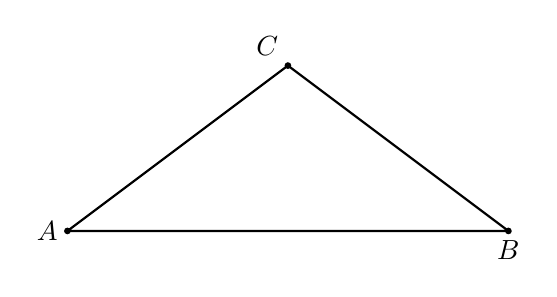
\begin{tikzpicture}[scale=0.7]
        \draw [<->, thick] (0,0)--(8,0)--(4,3)--cycle;
        \draw [fill] (0,0) circle [radius=0.05] node[left]{$A$};
        \draw [fill] (8,0) circle [radius=0.05] node[below]{$B$};
        \draw [fill] (4,3) circle [radius=0.05] node[above left]{$C$};
      \end{tikzpicture} \vspace{4cm}
    \end{center}
    \item What is the ratio of the \emph{area} of the dilated triangle to the original area of $\triangle ABC$? Justify your answer.
  \end{enumerate}

\newpage

Find the slope parallel and slope perpendicular to each linear equation.
    \begin{multicols}{2}
    \item   $y=\frac{3}{4}x-1$ \vspace{0.5cm}
      \begin{enumerate}
        \item   $m=$ \vspace{0.7cm}
        \item   $m_{\perp}=$ %\vspace{1cm}
      \end{enumerate}
    \item   $4-2y=6x$ \vspace{0.5cm}
      \begin{enumerate}
        \item   $m=$ \vspace{0.7cm}
        \item   $m_{\perp}=$ %\vspace{1cm}
      \end{enumerate}
    \end{multicols}

  \item Use slopes to prove that $\triangle ABC$ is a right triangle, given $A(-5,-2)$, $B(5,0)$, and $C(-1,4)$, as shown below.
    \begin{multicols}{2}
      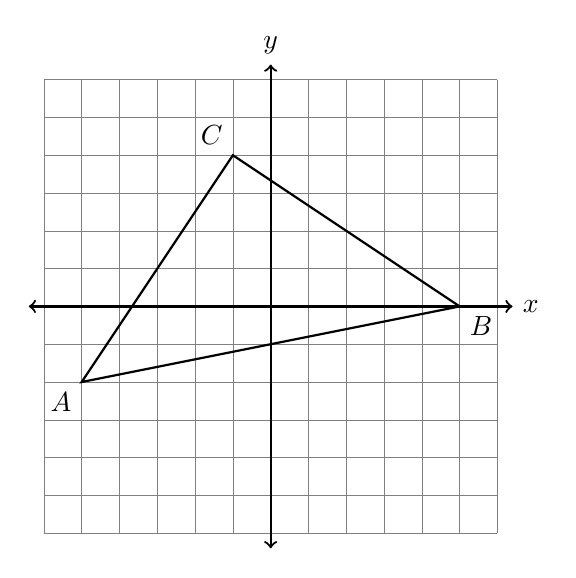
\begin{tikzpicture}[scale=.48]
        \draw [help lines] (-6,-6) grid (6,6);
        \draw [thick, <->] (-6.4,0) -- (6.4,0) node [right] {$x$};
        \draw [thick, <->] (0,-6.4)--(0,6.4) node [above] {$y$};
          \draw [thick]
          (-5,-2) node[below left] {$A$}--
          (5,0) node[below right] {$B$}--
          (-1,4) node[above left] {$C$}--
          cycle;
      \end{tikzpicture}
      Checklist. Confirm that you...
      \begin{itemize}
        \item Calculated the slopes of $\overline{AC}$ and $\overline{BC}$
        \item Showed that $m_{AC} \times m_{BC} = -1$
        \item Stated that therefore $\overline{AC} \perp \overline{BC}$
        \item Wrote a concluding statement, that therefore $\triangle ABC$ is a right triangle.
      \end{itemize}
    \end{multicols}

\newpage
 \item Point $M$ divides $\overline{AB}$ so that $AM{:}MB = 1{:}2$. If $A$ has coordinates $(-1,-5)$ and $B$ has coordinates $(5,4)$, what are the coordinates of $M$? \vspace{6cm}

 \item Triangle $ABC$ is inscribed in the semi-circle centered at $O$, with $m\angle C=90^\circ$, as shown. If $AC=8$ and $BC=15$, what is the radius of circle $O$? \vspace{0.5cm}
   \begin{center}
     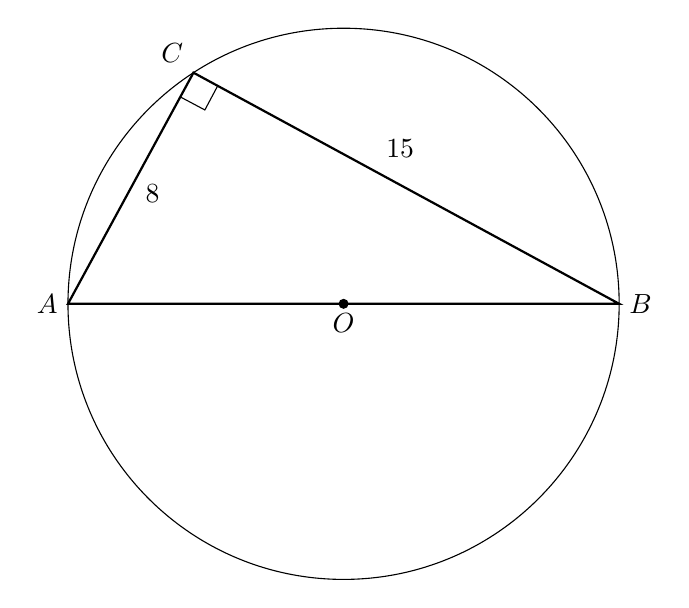
\begin{tikzpicture}[scale=0.7]
       \draw [<->, thick] (-5,0)node[left]{$A$}
       --(123:5)node[above left]{$C$}
       --(5,0)node[right]{$B$}--cycle;
       \draw (0,0) circle [radius=5] node[below]{$O$};
       \draw (123:5) ++(-28:0.5)-- ++(-118:0.5)-- +(152:0.5);
       \draw [fill] (0,0) circle [radius=0.08];
       \node at (70:3){15};
       \node at (150:4){8};
     \end{tikzpicture}
  \end{center}\vspace{5cm}


\end{enumerate}
\newpage
\setcounter{page}{1}
\subsubsection*{13.5 Exit Note: Construction \& graphing quiz}
Use only a compass and straightedge for these classical constructions, showing all construction marks.

  \begin{enumerate}
    \item Duplicate a given angle.\\[0.5cm]
    \hspace{1cm} Construct an angle with vertex $R$ and one leg the given ray $\overrightarrow{R}$, congruent to $\angle A$. Show all construction marks.
      \vspace{1cm}
      \begin{center}
      \begin{tikzpicture}
        \draw [<->, thick] (3,6)--(0,0)--(9,0);
        \draw [fill] (0,0) circle [radius=0.05] node[below]{$A$};
        \draw [->, thick] (2,-9)--(10,-9);
        \draw [fill] (2,-9) circle [radius=0.05] node[below]{$R$};
      \end{tikzpicture}
      \end{center}

\newpage
  \item Construct point $B'$ on the ray $l$ such that $\overline{AB} \cong \overline{A'B'}$.
      \vspace{1cm}
      \begin{center}
      \begin{tikzpicture}
        \draw [-, thick] (0,0)--(4,0);
        \draw [->, thick] (2,-2)--(10,-2);
        \draw [fill] (2,-2) circle [radius=0.05] node[above left]{$A'$};
        \draw [fill] (0,0) circle [radius=0.05] node[above left]{$A$};
        \node at (8.5,-2)[below]{$l$};
        \draw [fill] (4,0) circle [radius=0.05] node[above right]{$B$};
      \end{tikzpicture}
      \end{center}
      \vspace{1.5cm}

  \item
  \begin{enumerate}
    \item Dilate $\triangle ABC$ by a factor of $k=2$ centered at $A$.\\[0.5cm]
  (hint: extend $\overrightarrow{AB}$ and $\overrightarrow{AC}$, then duplicate $\overline{AB}$ and $\overline{AC}$.)\\[3cm]
    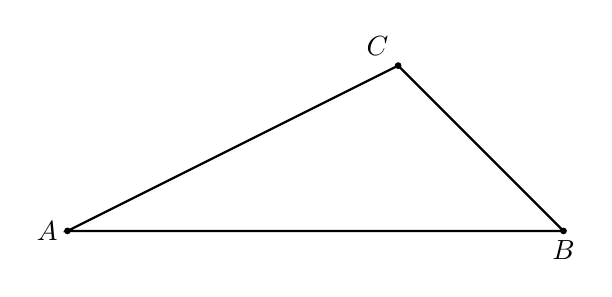
\begin{tikzpicture}[scale=0.7]
      \draw [<->, thick] (0,0)--(9,0)--(6,3)--cycle;
      \draw [fill] (0,0) circle [radius=0.05] node[left]{$A$};
      \draw [fill] (9,0) circle [radius=0.05] node[below]{$B$};
      \draw [fill] (6,3) circle [radius=0.05] node[above left]{$C$};
    \end{tikzpicture} \vspace{2cm}
    \item What is the ratio of the \emph{area} of the dilated triangle to the original area of $\triangle ABC$? Justify your answer.
  \end{enumerate}

\newpage

Find the slope parallel and slope perpendicular to each linear equation.
    \begin{multicols}{2}
    \item   $y=-\frac{2}{3}x+2$ \vspace{0.5cm}
      \begin{enumerate}
        \item   $m=$ \vspace{0.7cm}
        \item   $m_{\perp}=$ %\vspace{1cm}
      \end{enumerate}
    \item   $3+4y=2x$ \vspace{0.5cm}
      \begin{enumerate}
        \item   $m=$ \vspace{0.7cm}
        \item   $m_{\perp}=$ %\vspace{1cm}
      \end{enumerate}
    \end{multicols}

  \item Use slopes to prove that $\triangle ABC$ is a right triangle, given $A(-5,3)$, $B(4,-4)$, and $C(1,5)$, as shown below.
    \begin{multicols}{2}
      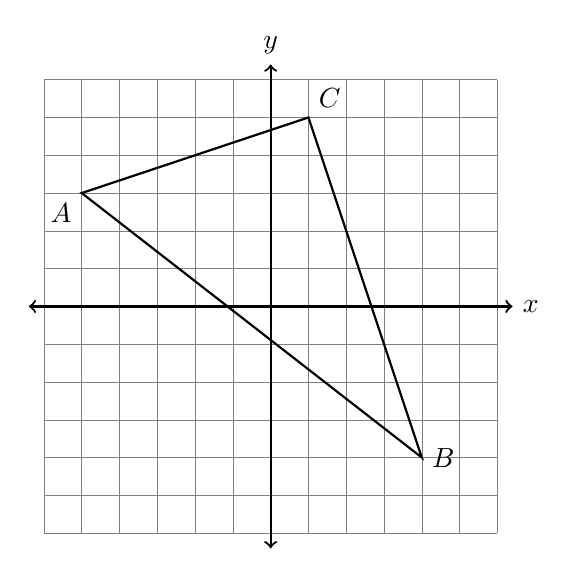
\begin{tikzpicture}[scale=.48]
        \draw [help lines] (-6,-6) grid (6,6);
        \draw [thick, <->] (-6.4,0) -- (6.4,0) node [right] {$x$};
        \draw [thick, <->] (0,-6.4)--(0,6.4) node [above] {$y$};
          \draw [thick]
          (-5,3) node[below left] {$A$}--
          (4,-4) node[right] {$B$}--
          (1,5) node[above right] {$C$}--
          cycle;
      \end{tikzpicture}
      Checklist. Confirm that you...
      \begin{itemize}
        \item Calculated the slopes of $\overline{AC}$ and $\overline{BC}$
        \item Showed that $m_{AC} \times m_{BC} = -1$
        \item Stated that therefore $\overline{AC} \perp \overline{BC}$
        \item Wrote a concluding statement, that therefore $\triangle ABC$ is a right triangle.
      \end{itemize}
    \end{multicols}

\newpage
 \item Point $M$ divides $\overline{AB}$ so that $AM{:}MB = 1{:}2$. If $A$ has coordinates $(-2,-4)$ and $B$ has coordinates $(7,8)$, what are the coordinates of $M$? \vspace{6cm}

 \item Triangle $ABC$ is inscribed in the semi-circle centered at $O$, with $m\angle C=90^\circ$, as shown. If $AC=12$ and $BC=5$, what is the radius of circle $O$? \vspace{0.5cm}
   \begin{center}
     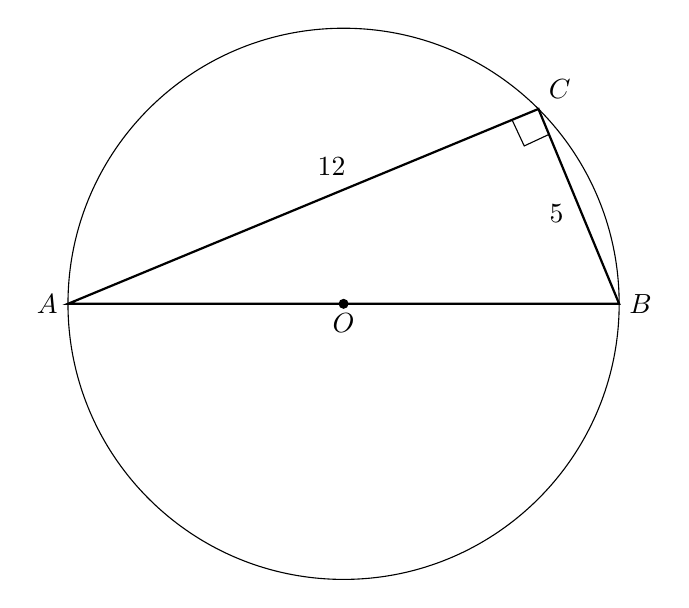
\begin{tikzpicture}[scale=0.7]
       \draw [<->, thick] (-5,0)node[left]{$A$}
       --(45:5)node[above right]{$C$}
       --(5,0)node[right]{$B$}--cycle;
       \draw (0,0) circle [radius=5] node[below]{$O$};
       \draw (45:5) ++(-67:0.5)-- ++(-155:0.5)-- +(115:0.5);
       \draw [fill] (0,0) circle [radius=0.08];
       \node at (95:2.5){12};
       \node at (23:4.2){5};
     \end{tikzpicture}
  \end{center}\vspace{5cm}

\end{enumerate}
\end{document}
